\documentclass[onecolumn]{aastex62}


\newcommand{\vdag}{(v)^\dagger}
\newcommand\aastex{AAS\TeX}
\newcommand\latex{La\TeX}
\usepackage{listings}
\usepackage{amsmath}
\usepackage{physics}
\usepackage{hyperref}
\usepackage{natbib}
\usepackage[T1]{fontenc}
\usepackage[english]{babel}
\usepackage[utf8]{inputenc}

\begin{document}

\title{\Large Milestone IV:\\Computing the CMB power spectrum.}

\author{Håkon Tansem}

\section{Introduction} \label{sec:intro}
This is the fourth and last milestone in a four milestone project where the end goal is to compute the CMB power spectrum. We have previously studied the expansion history of the universe and the recombination history culminating in calculating and studying the evolution of the initial perturbations given by the Einstein and Boltzmann equations. In this last milestone we will combine the knowledge gained from the previous three milestones and finally compute the CMB power spectrum. We will also use our computed parameters to calculate the matter power spectrum to study how matter overdensities have evolved for different cosmic scales.
\section{Method} \label{sec:method}
The CMB temperature field is given by
\begin{equation}
    T(\hat{n}) = \sum_{\ell m} a_{\ell m} Y_{\ell m}(\hat{n}),
\end{equation}
where $\hat{n}$ is the direction on the sky, $Y_{\ell m}$ is the spherical harmonics and $a_{\ell m}$ is coefficient of the spherical harmonics. We want to study which scales are most influential when studying the sky map. This is defined by the CMB power spectrum given by 
\begin{equation}
    C_\ell \equiv \langle |a_{\ell m}|^2 \rangle = \langle a_{\ell m}a_{\ell m}^* \rangle.
\end{equation}
In Milestone III, we computed the evolution of the temperature field $\theta_\ell(k)$ for $\ell=0$ up to $\ell=6$. We want to know the value of the temperature field today at $x=0$. In order to compute a reasonable portion of the power spectrum, so that we can study the most important effects, we need multipoles up to at least $\ell=1200$. This would make the system of equations in Milestone III very large. This is when we will use a method called line of sight integration developed by Zaldarriaga and Seljak. For a brief derivation of this, see \cite{callin2006calculate:2006}. The basic idea behind this is to 
start with the expression for $\frac{d\theta}{dx}$, integrate it and then expand in multipoles at the end. This gives us the integral
\begin{equation}\label{eq:theta_int}
    \Theta_\ell(k, x=0) = \int_{-\infty}^{0} \tilde{S}(k,x)
              j_\ell[k(\eta_0-\eta)] dx,
\end{equation}
where $j_\ell$ is the spherical bessel function and $\tilde{S}(k,x)$ is the source function given by
\begin{equation}
    \tilde{S}(k,x) = \tilde{g}\left[ \Theta_0 + \Psi + \frac{1}{4}\theta_2\right] +
              e^{-\tau} \left[\Psi^\prime-\Phi^\prime\right] -
              \frac{1}{ck}\frac{d}{dx}(\mathcal{H}\tilde{g}v_b) + \frac{3}{4c^2k^2} \frac{d}{dx}
              \left[\mathcal{H}\frac{d}{dx} (\mathcal{H}\tilde{g}\theta_2)\right]
\end{equation}
\cite{WintherIV:2020}. (Beskriv leddene?) All parameters in the source function are explained in the earlier milestones. The spherical bessel function has been pre-calculated for arguments between $0$ and $5000$ with $10000$ linearly space points between them for every ell used in the integral and then splined. This allows us to evaluate the bessel function for all arbitrary $k(\eta_0-\eta)$ values for every $\ell$ we have created a spline for. In our model the integral in equation \ref{eq:theta_int} will be implemented as an ODE given as
\begin{equation}\label{eq:theta_ODE}
    \frac{d\Theta_\ell(k, x)}{dx} = \tilde{S}(k,x) j_\ell[k(\eta_0-\eta)],\,\,\, \Theta_\ell(k, -\infty) = 0.
\end{equation}
This equation is then solved for every $k$ in a logarithmically spaced grid with $k_{min}=0.00001/$Mpc and $k_{max}=0.1/$Mpc with $2000$ values and for every k we solve for $63$ relatively evenly distributed $\ell$ values between $2$ and $2000$. The solution is then splined so that we can evaluate $\theta_\ell(k)$ for all $\ell$ values we used and an arbitrary $k$ in the interval we used to solve the ODE. Now that we have the actual temperature field $\theta_\ell(k)$ we can start solving for the power spectrum $C_\ell$. The $C_\ell$ will be an integral over the fourier coefficients $\theta_\ell$ squared, as well as the primordial power spectrum $P_{primordial}(k)$. This gives us the integral for $C_\ell$
\begin{equation}
    C_\ell = \frac{2}{\pi}\int k^2P_{\rm primordial}(k) \Theta_\ell^2(k)dk.
\end{equation}
The primordial power spectrum is given as
\begin{equation}
    \frac{k^3}{2\pi^2} P_{\rm primordial}(k) = A_s \left(\frac{k}{k_{\rm pivot}}\right)^{n_s-1},
\end{equation}
where $n_s$ is the spectral index which we set $n_s=0.96$ $k_{\rm pivot}$ is a scale with a given amplitude $A_s$. In our model we will use $k_{\rm pivot} = 0.05/$Mpc and $A_s=10^{-9}$. This gives our final expression for $C_\ell$ aasjournal
\begin{equation}\label{eq:Cell_int}
    C_\ell = 4\pi \int_0^{\infty} A_s \left(\frac{k}{k_{\rm pivot}}\right)^{n_s-1} \Theta_{\ell}^2(k) \frac{dk}{k}
\end{equation}
\cite{WintherIV:2020}. In our model we will solve this, like we did with $\theta_{\ell}(k)$, using and ODE approach rewriting the integral in equation \ref{eq:Cell_int} to 
\begin{equation}\label{eq:Cell_ODE}
    \frac{dC_{\ell}}{dlogk} = 4 \pi P_{\rm primordial}(k) \theta_{\ell}(k)^2.
\end{equation}
This equation is solved Using the same $k$-values and $\ell$ as for the $\theta_{\ell}(k)$ ODE given in equation \ref{eq:theta_ODE}. The result is then splined so that we now can evaluate $C_{\ell}$ for every every between $2$ and $2000$.
\section{Results}
\label{sec:results}
All results were produced using a comsology with the following parameters $h =
0.7,\,\,\,T_{\rm CMB 0} = 2.725,\,\,\,\Omega_{r0} = 5.046\cdot
10^{-5},\,\,\,\Omega_{b0}=0.046,\,\,\,\Omega_{\rm CDM 0} =
0.224,\,\,\,\Omega_{\Lambda 0} = 0.72995,\,\,\,\Omega_{k0} = \Omega_{\nu 0} =
0$. When plotting the $C_\ell$ values for the temperature power spectrum our
model produced the result illustrated in figure \ref{fig:cell}. In this figure
we have inclued the Planck public release data 1 from 2013 to compare with our
model. For the Planck data we have neglected corresponding error bars and
uncerertainties in the data set as plotting this data is meant as a rough
comparison to our model. The transfer function $\theta_\ell(k)$ is illustrated
in figure \ref{fig:transfer}. Here we we chose to illustrate $/ell=200$ and
$\ell=350$ as this approximately corresponds to the first peak and through of
our temperature power spectrum. We also included $/ell=6$ and $\ell=1600$ to see
the difference on vastly different scales. The spectrum integrand
$\theta_\ell(k)^2/k$ is shown in figure \ref{fig:integrand} for the same
multipole values as in figure \ref{fig:transfer} excluding $\ell=6$ as this had
a significantly larger amplitude than the other multipole values.\\
\begin{figure}
    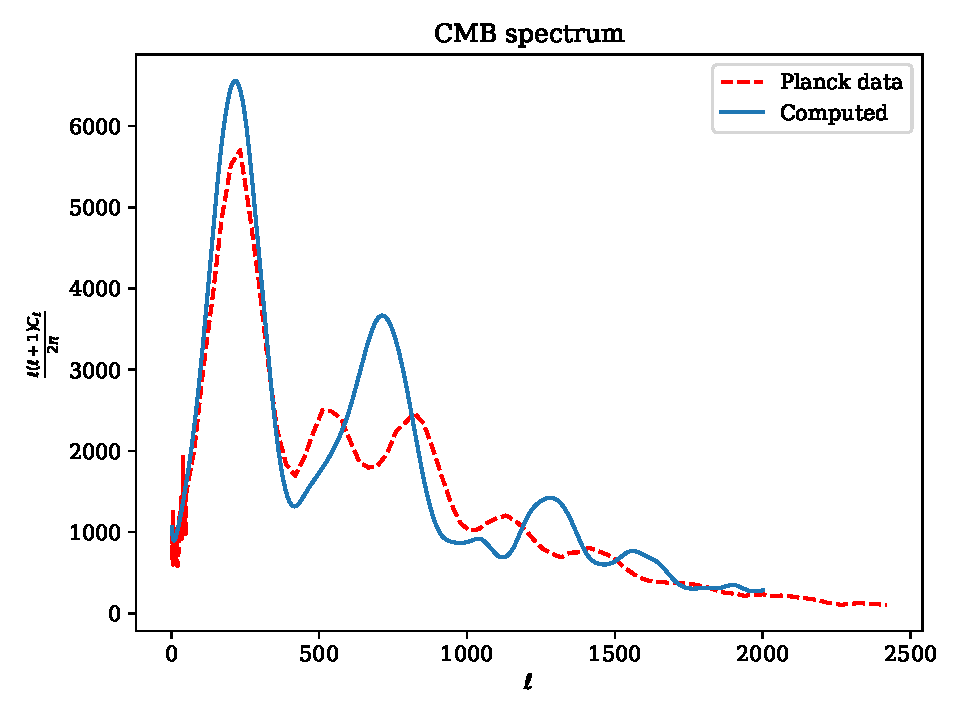
\includegraphics[scale=0.8]{figures/comparison.pdf}
    \caption{The top figure shows the computed CMB temperature power-spectrum. The bottom figure shows the computed powerspectrum along with the planck public release data 1. For the planck data we have neglected error bars in the data set as this plot is just to roughly compare our computed spectrum with the measured power-spectrum.}
    \label{fig:cell}
\end{figure}
\begin{figure}
    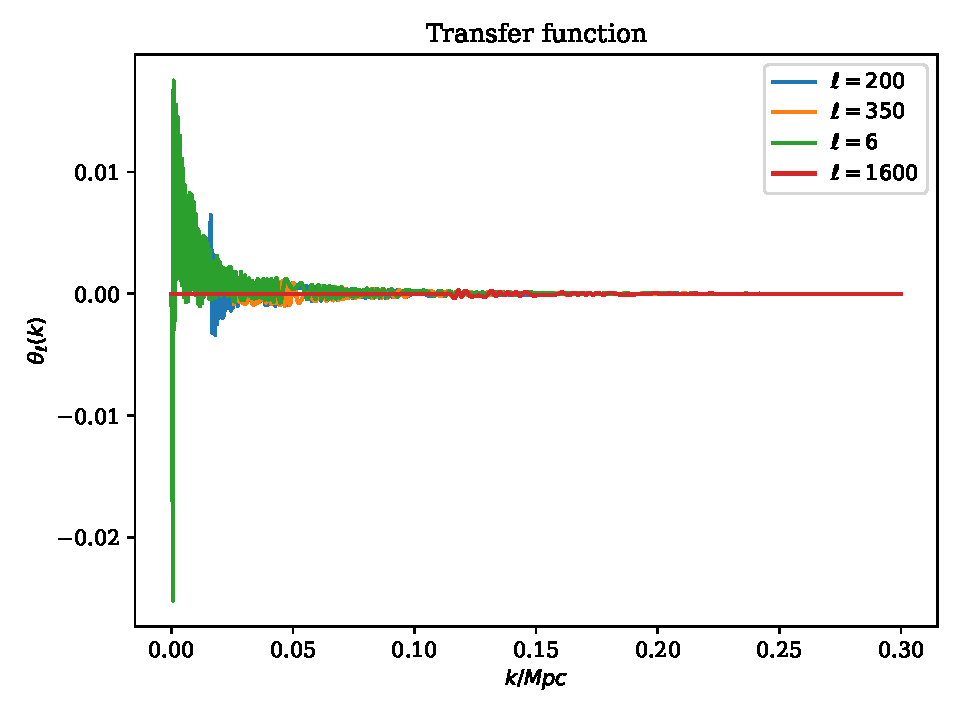
\includegraphics[scale=0.8]{figures/transfer.pdf}
    \caption{Figure showing the transfer function $\theta_\ell(k)$ for four different scales. The scales $/ell=200$ and
    $\ell=350$ were chosen as they approximately corresponds to the first peak and through of
    our temperature power spectrum. $/ell=6$ and $\ell=1600$ were chosen to
    illustrate the difference between vastly different scales.}
    \label{fig:transfer}
\end{figure}
\begin{figure}
    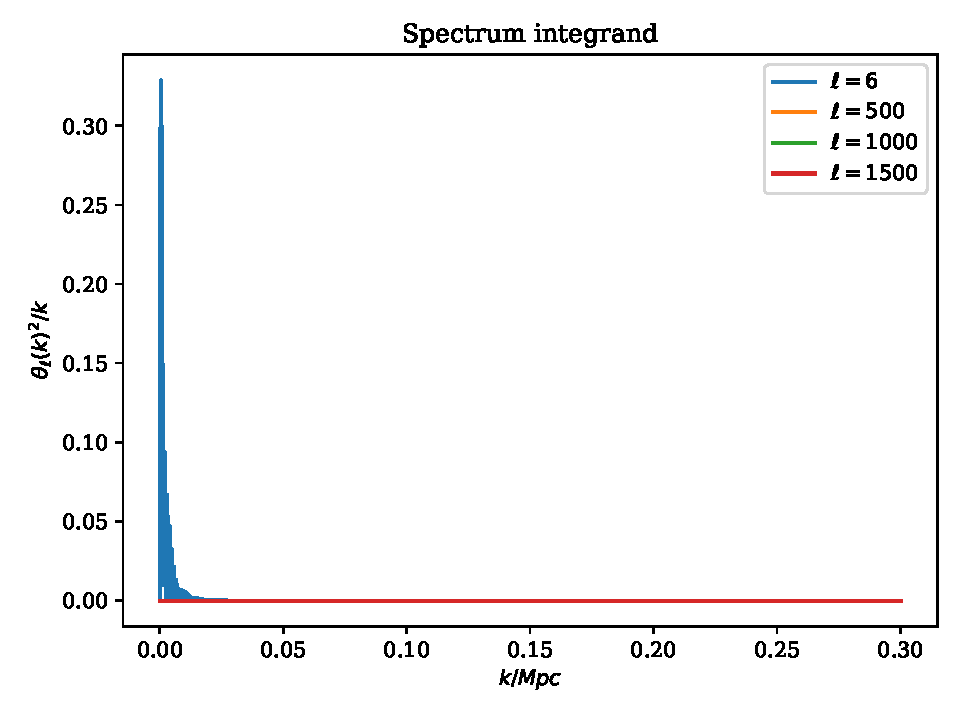
\includegraphics[scale=0.8]{figures/integrand.pdf}
    \caption{Figure showing the spectrum integrand$\theta_\ell(k)^2/k$ for three different scales.}
    \label{fig:integrand}
\end{figure}

The matter power spectrum given in by equation (eq) is given in figure \ref{fig:matter}
\begin{figure}
    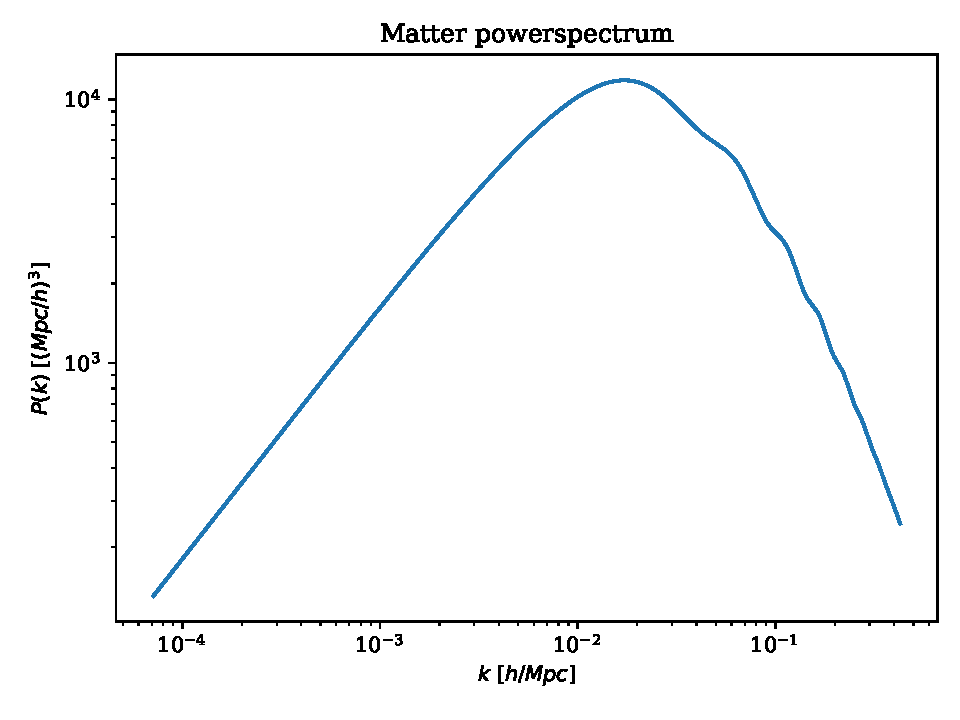
\includegraphics[scale=0.8]{figures/P.pdf}
    \caption{Figure showing the matter power spectrum $P(k)$. Here $k_{peak}$ is plotted as this marks the extremal point in the matter power-spectrum denoting the turnover between supressed scales and non supressed scales.}
    \label{fig:matter}
\end{figure}

\section{Discussion}\label{sec:discussion}

\bibliography{ref.bib}
\bibliographystyle{aasjournal}
%\begin{thebibliography}{}
%\end{thebibliography}
\end{document}

% End of file `sample62.tex'.
